\documentclass{article}
\usepackage[utf8]{inputenc}
\usepackage{geometry}
\usepackage{hyperref}
\usepackage{graphicx}
\usepackage{longtable}
\usepackage{hyperref}
\usepackage{graphicx}
\usepackage{xcolor}
\geometry{a4paper, margin=1in}

\title{Einrichtungsanweisungen \\Jetson Orin Nano Developer Kit}
\author{}
\date{}

\begin{document}

\maketitle

\section*{Einleitung}

Das NVIDIA\textsuperscript{\textregistered} Jetson Orin Nano\textsuperscript{\texttrademark} Developer Kit ermöglicht die Entwicklung von KI-gesteuerten Robotern, intelligenten Drohnen und intelligenten Kameras basierend auf der Jetson Orin Nano-Serie.

\begin{figure}[h!]
    \centering

    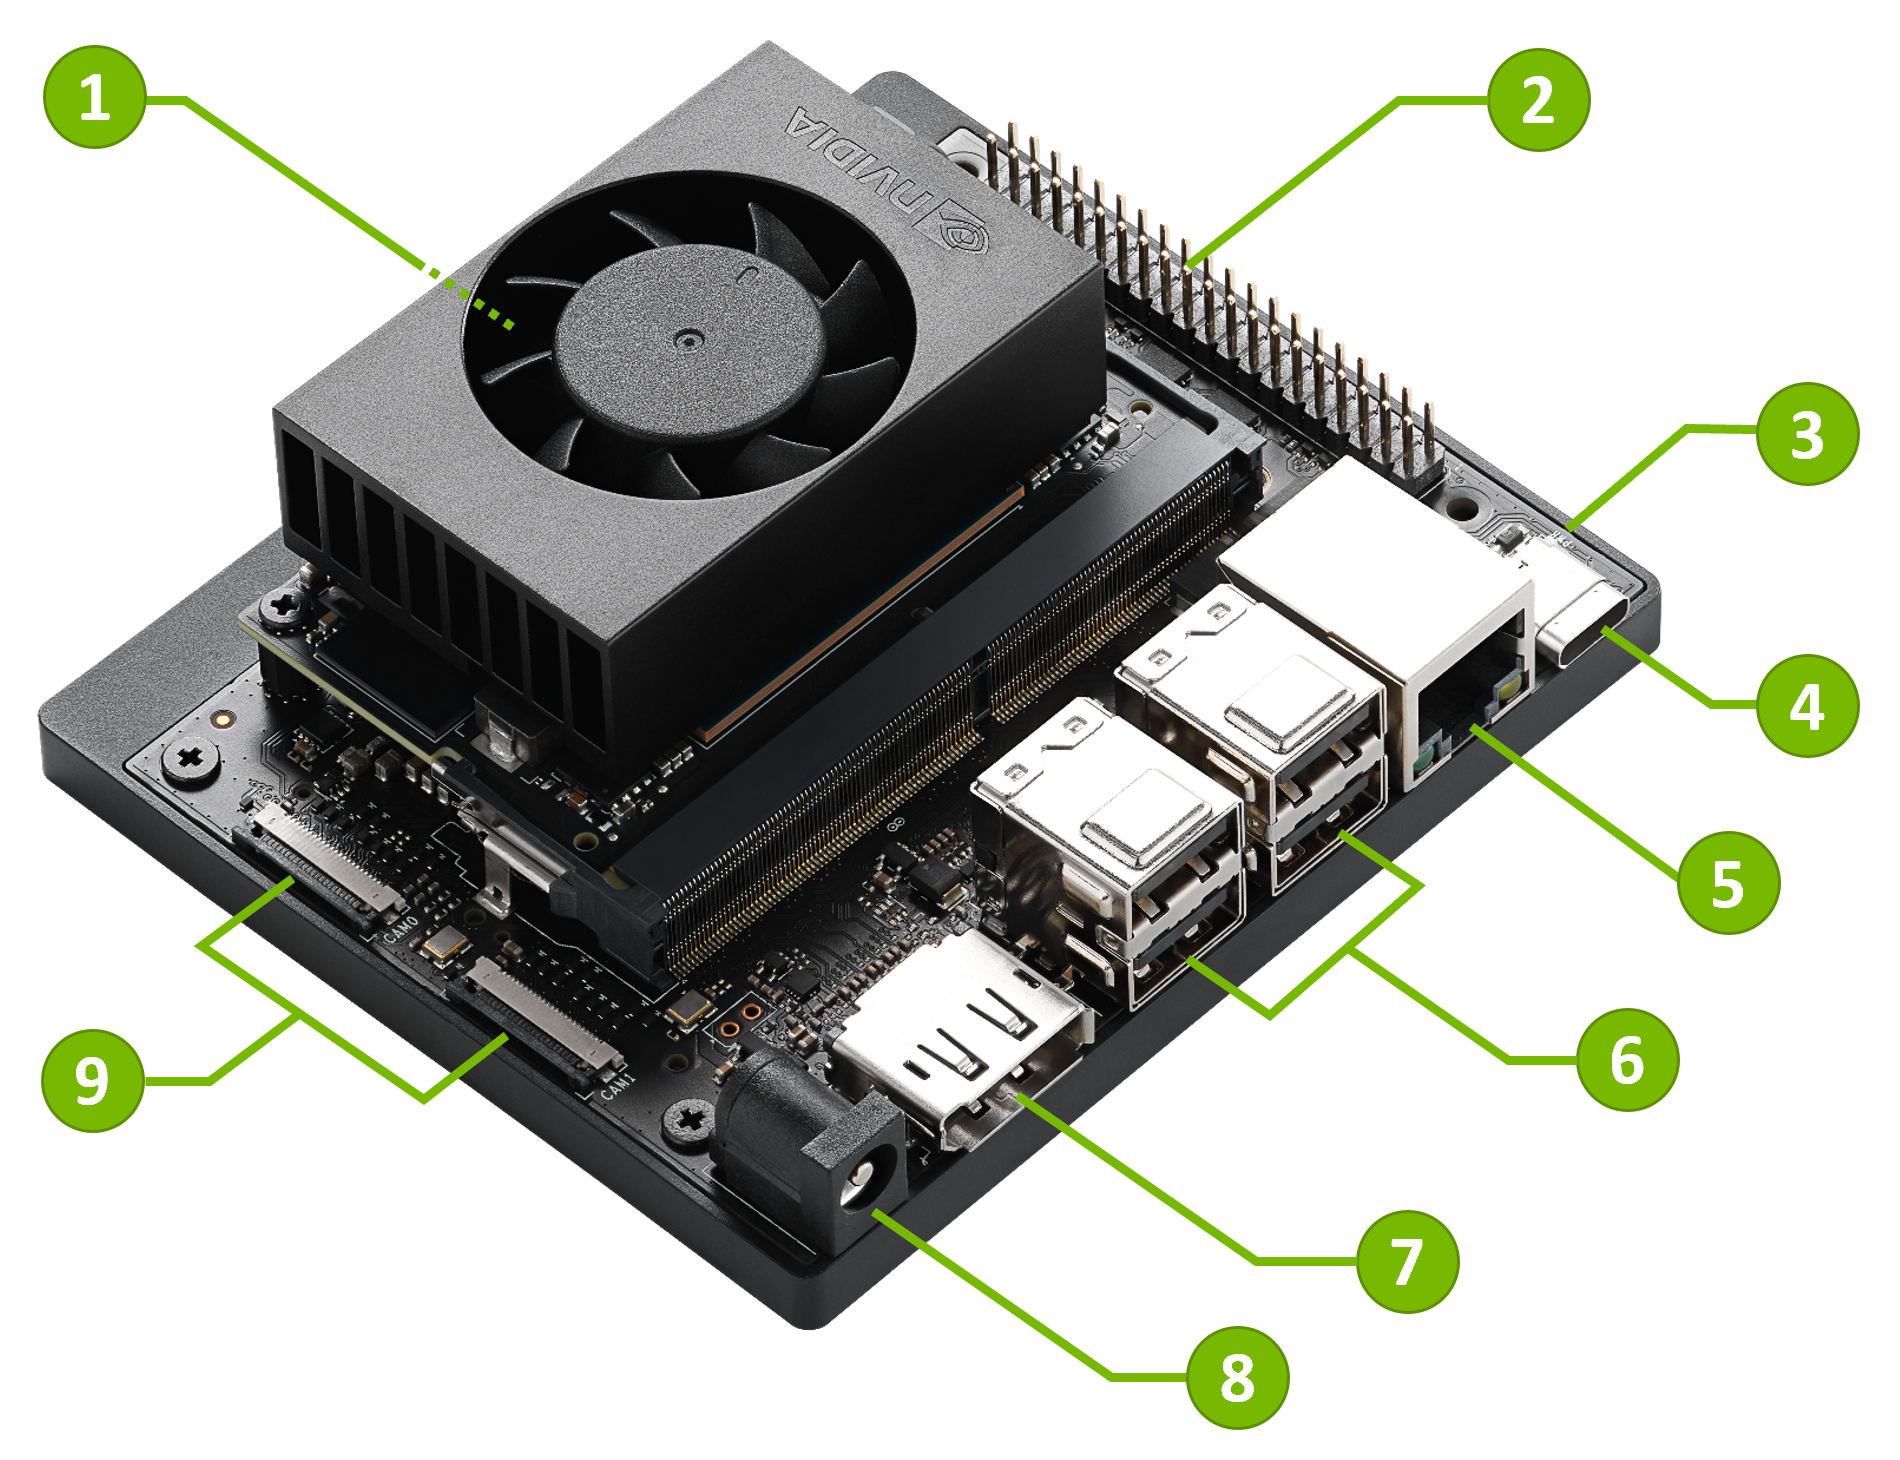
\includegraphics[width=0.8\textwidth]{jetsonOrinNano8GB.png} 

    \caption{Jetson Orin Nano Developer Kit}
\end{figure}

\subsection*{Merkmale}

\begin{itemize}
    \item microSD-Kartensteckplatz für den Hauptspeicher
    \item 40-poliger Erweiterungsheader
    \item Stromanzeigen-LED
    \item USB-C-Port nur für Daten
    \item Gigabit-Ethernet-Port
    \item USB 3.1 Typ A Ports (x4)
    \item DisplayPort-Anschluss
    \item DC Barrel Jack für 19V Stromversorgung
    \item MIPI CSI Kameraanschlüsse
\end{itemize}

\subsection*{Im Lieferumfang enthalten}

\begin{itemize}
    \item Jetson Orin Nano Modul mit microSD-Kartensteckplatz
    \item Referenzträgerplatine (inklusive 802.11 Plug-in WLAN \& BT-Modul vorinstalliert mit Antenne)
    \item 19V Netzteil
    \item Eine kleine Papierkarte mit Schnellstart- und Support-Informationen
\end{itemize}

\subsection*{Nicht im Lieferumfang enthalten}

\begin{itemize}
    \item microSD-Karte (empfohlen 64GB UHS-1 oder größer)
    \item USB-Tastatur und Maus
    \item Computerbildschirm
    \item USB-Kabel
    \item Zunächst ist ein Computer mit Internetverbindung und der Fähigkeit zum Flashen der microSD-Karte ebenfalls erforderlich.
\end{itemize}
\newpage
\section*{Firmware aktualisieren (falls erforderlich)}

Ihr Jetson Orin Nano Developer Kit ist möglicherweise bereits bereit, JetPack 6 auszuführen, da die neueste Firmware (\textit{Jetson UEFI Firmware} auf QSPI-NOR Flash-Speicher) ab Werk geflasht wurde.

Falls dies nicht der Fall ist, müssen Sie auf die neueste Firmware aktualisieren.

Sie können nun die neueste Firmware auf Jetson aktualisieren, ohne einen Host-Ubuntu-PC zu benötigen: Befolgen Sie die Schritte auf dieser \textcolor{blue}{\href{https://www.jetson-ai-lab.com/initial_setup_jon.html}{Seite}}, um zu überprüfen, ob Ihr Jetson Orin Nano Developer Kit die neueste Firmware hat, und aktualisieren Sie diese mit einer SD-Karte, die JetPack 5 enthält.

Folgen Sie den Anweisungen \textcolor{blue}{\href{https://www.jetson-ai-lab.com/initial_setup_jon.html}{hier}}.

Sobald Sie bestätigt haben, dass Ihr Jetson Orin Nano Developer Kit die neueste Firmware hat, die JetPack 6 ausführen kann, fahren Sie mit dem nächsten Schritt fort.


\newpage
\section{Image auf die microSD-Karte schreiben}

Um Ihr Jetson Orin Nano Developer Kit einzurichten, müssen Sie die microSD-Karte mit dem richtigen Image vorbereiten. Folgen Sie diesen Schritten:

\subsection{Das Jetson Orin Nano Developer Kit-Image herunterladen}
\begin{itemize}
    \item Besuchen Sie das \href{https://developer.nvidia.com/embedded/downloads}{Jetson Download Center} und laden Sie das neueste SD-Karten-Image herunter.
    \item Die heruntergeladene Datei liegt normalerweise im \texttt{.zip}-Format vor. Entpacken Sie die Datei, um die \texttt{.img}-Datei zu erhalten.
\end{itemize}

\subsection{microSD-Karte in den Host-Computer einlegen}
\begin{itemize}
    \item Verwenden Sie einen microSD-Kartenleser, um die Karte in Ihren Computer einzulegen.
    \item Stellen Sie sicher, dass die microSD-Karte von Ihrem Betriebssystem erkannt wird.
\end{itemize}

\subsection{Nutzen Sie SD Card Formatter, um die SD Karte zu formatieren.}
\begin{center}
    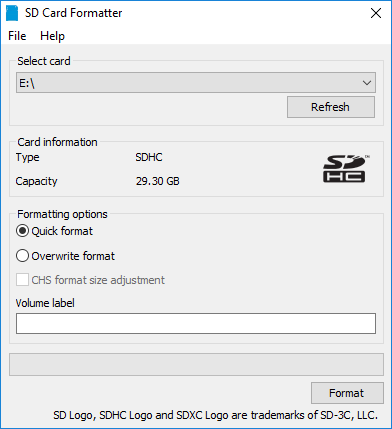
\includegraphics[width=0.8\textwidth ]{SD_Card_Formatter.png}
\end{center}

\begin{itemize}
    \item Laden und führen Sie die \textcolor{blue}{\href{https://www.sdcard.org/downloads/formatter/sd-memory-card-formatter-for-windows-download/}{SD Memory Card Formatter for Windows}} aus.
    \item Wählen Sie das Kartenlaufwerk aus.
    \item Wählen Sie``Schnellformatierung''.
    \item Lassen Sie ``Volume-Label'' leer.
    \item Klicken Sie auf ``Formatieren'', um mit dem Formatieren zu beginnen, und bestätigen Sie mit ``Ja'' im Warn-Dialog.
\end{itemize}
\subsection{4. Image auf die microSD-Karte schreiben}
\begin{itemize}
    \item Nutzen Sie ein Tool wie Balena Etcher, das für Windows, Mac und Linux verfügbar ist.
\end{itemize}

\textbf{Schritte mit Balena Etcher:}
\begin{enumerate}
    \item Installieren und öffnen Sie \textcolor{blue}{\href{https://etcher.balena.io/}{Balena Etcher.}}
    \begin{center}
        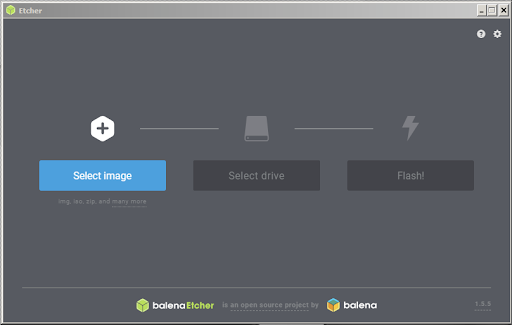
\includegraphics[width=0.8\textwidth ]{Etcher.png}
    \end{center}
    \item Wählen Sie die entpackte \texttt{.img}-Datei aus.
    \item Wählen Sie die microSD-Karte als Zielgerät aus.
    \begin{center}
        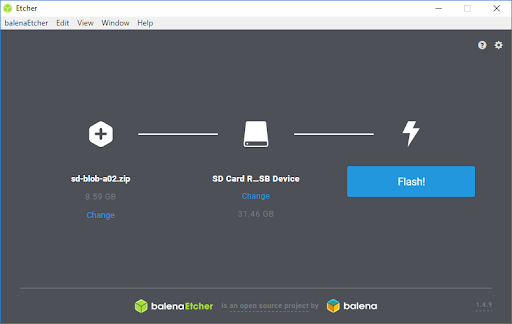
\includegraphics[width=0.8\textwidth ]{Etcher_Select_Drive.png}
    \end{center}
    \item Klicken Sie auf die Schaltfläche \textquotedblleft Flash\textquotedblright, um das Image auf die Karte zu schreiben.
\end{enumerate}

\subsection{4. Image überprüfen}
\begin{itemize}
    \item Balena Etcher überprüft automatisch die geschriebenen Daten.
    \item Wenn die Überprüfung fehlschlägt, wiederholen Sie den Flash-Vorgang oder verwenden Sie eine andere microSD-Karte.
\end{itemize}

\subsection{5. microSD-Karte sicher entfernen}
\begin{itemize}
    \item Werfen Sie die microSD-Karte sicher aus, um Datenbeschädigungen zu vermeiden.
\end{itemize}

\newpage
\section{Einrichtung und erster Start}

\subsection{1. Verbindungen herstellen}
\begin{itemize}
    \item \textbf{microSD-Karte einlegen:} Setzen Sie die vorbereitete microSD-Karte ein.
    \item \textbf{Peripheriegeräte anschließen:} USB-Tastatur, Maus und Monitor.
    \item \textbf{Netzwerkverbindung herstellen:} Ethernet-Kabel anschließen.
    \item \textbf{Stromversorgung anschließen:} 19V-Netzteil mit dem DC-Eingang verbinden.
\end{itemize}

\subsection{2. Erster Start}
\begin{itemize}
    \item Das Developer Kit startet automatisch. Die grüne LED leuchtet.
    \item Folgen Sie den Anweisungen zur Einrichtung (EULA, Sprache, Zeitzone, WLAN, Benutzerkonto).
\end{itemize}

\subsection{3. Nach dem Login}
\begin{verbatim}
sudo apt update
sudo apt upgrade
\end{verbatim}

\section{Nächste Schritte}
\begin{itemize}
    \item Verwenden Sie den Jetson SDK Manager, um zusätzliche NVIDIA-Softwarepakete zu installieren.
    \item Besuchen Sie die NVIDIA Developer Website für Tutorials und Beispiele.
\end{itemize}

\section{Technische Spezifikationen}

\subsection{Prozessor (CPU)}
\begin{itemize}
    \item \textbf{Architektur:} ARM Cortex-A78AE
    \item \textbf{Kerne:} 6 Kerne, bis zu 1,5 GHz
\end{itemize}

\subsection{Grafikprozessor (GPU)}
\begin{itemize}
    \item \textbf{Architektur:} NVIDIA Ampere, 64 Tensor Cores, 40 TOPS
\end{itemize}

\subsection{Speicher (RAM)}
\begin{itemize}
    \item 4 GB oder 8 GB LPDDR5, bis zu 68 GB/s Bandbreite
\end{itemize}

\subsection{Schnittstellen und I/O}
\begin{itemize}
    \item PCIe Gen 3 x4, USB 3.2, Gigabit-Ethernet
    \item HDMI 2.1, DP 1.2, 2x MIPI CSI-2 Kameraanschlüsse
\end{itemize}

\subsection{Leistung und Energieverbrauch}
\begin{itemize}
    \item Einstellbarer Energieverbrauch: 7 W bis 15 W
\end{itemize}

\subsection{Softwareunterstützung}
\begin{itemize}
    \item Linux for Tegra (L4T), Unterstützung für CUDA 11, C++, Python, TensorFlow, PyTorch
\end{itemize}

\section{Vergleich der Modelle}

\begin{longtable}{|l|c|c|c|}
    \hline
    \textbf{Modell} & \textbf{RAM} & \textbf{Leistung (TOPS)} & \textbf{Energieverbrauch} \\
    \hline
    Jetson Orin Nano 4GB & 4 GB & 20 TOPS & 7–15 W \\
    Jetson Orin Nano 8GB & 8 GB & 40 TOPS & 7–15 W \\
    \hline
\end{longtable}

\end{document}
